\documentclass{article}

\usepackage[margin=1.0in]{geometry}
\usepackage{graphicx}
\usepackage{amsmath}
\usepackage{float}
\usepackage{enumitem}

\title{CSC 535 HW7}
\date{11/15/2018}
\author{Simon Swenson}

\begin{document}

\pagenumbering{gobble}
\maketitle
\pagenumbering{arabic}

\large Introduction

\small I completed all required homework problems. Question 1 took me quite a 
while because I was trying to create a general solution without fully 
understanding the solution completely. Instead, I created a more specific solution that only applies to MQLs. This also 
gave me a concrete example to help me better understand the message passing 
process. After I switched to the more specific implementation, work went much 
faster, and I completed that question in about 10\% of the time that I had spent 
working on the general solution.

You might have also noticed that I have moved 
to using Python and Numpy in these coding assignments. This is due to a couple 
of reasons. First, I am more familiar with it, which is not a great excuse, but 
I have been pretty busy during this part of the semester, and I would rather spend 
more time working through the material than struggling through syntax. Second, 
Python is better integrated into Linux. Matlab uses a monolithic binary that I 
cannot install through my package manager. This causes the suite to have a fair 
bit of bloat on my machine. I could work through it at this point in time, but I 
am definitely pushing 
the bounds on my fairly low-end laptop in multiple ways, including storage 
space. If you think I should still stick with Matlab, let me know, and I will switch back.


On another note, sorry about the hand-drawn 
graphs in the previous couple of assignments. I had been making graphs in 
Inkscape previously, but, I was strapped for time, so I reverted to the 
hand-drawn graphics. I'll stick to the computer-drawn graphics from now on.

\section{Q1}

Previously, we had been exploring the structure of PGMs and the 
generation of data points from the distributions, there is a clever and (fairly) 
straightfoward way to predict using factor graphs. However, an equally important 
question in the field of machine learning is classification. That is, given a 
data point and a model, can we use the model to predict the class of the data 
point? In the case of PGMs, we use a factor graph and implement the sum-product 
algorithm via message passing on it to perform classification. Intuitively, the 
message passing is figuring out the distributions for the hidden, underlying values, 
given noisy observations. For example, in the case of MQLs, we know that an observed outer 
right arm angle of 8 could not have been produced by an actual outer right arm 
angle of 4, since the underlying noise distribution, P(ooraa = 8 | oraa = 4) = 0. 
We actually get more information than that: We get a probability distribution 
for what the child thinks about the parent's possible variable values. This is 
done in the factor nodes, via matrix multiplication.
In addition, we can consult mutiple incoming factors to find out where they 
actually agree on their hypothesized distributions. This is represented by the 
work of the value nodes, an element-wise multiplcation, which only keeps 
possibilities where all factors have a non-zero probability.

The actual algorithm is provided in the accompanying hw7.py. It is a fairly 
simple sum-product algorithm, specific to MQLs. Note 
that it makes use of pre-computed matrices and performs most of the heavy 
lifting by multiplying vectors with those matrices. Performance is better than 
chance. I am getting around 85\% accuracy on a sample size of 10,000. Comparing 
to a baseline, The chance performance in this case is actually ~67\%, since the 
prior distribution of sex is ~67\% male and ~33\% female. Thus, you could create 
a classifier that always votes for male and still achieve 67\% accuracy.

\section{Q2}

\begin{figure}[!ht]
	\centering
	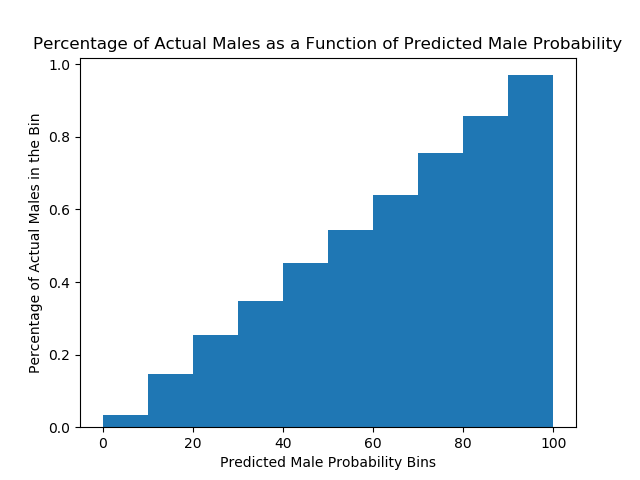
\includegraphics[width=120mm]{figs/Q2.png}
	\caption{The number of actual males in each bin correlates linearly with the 
        model's predicted male probability. This seems to indicate that 
        the model learns a linear separator. Indeed, the implementation is a 
        series of linear operations on matrices and vectors, so this is actually 
        not too surprising. It is a bit disappointing, however, as nonlinear 
        classifiers are much more powerful. However, we may be able to 
        incorporate a kernel trick to transform the input space. One caveat of 
        going down that path, however, is that we lose a lot of sensible meaning 
        from the graph. Furthermore, it is not intuitively obvious how to 
        construct a graph from the new feature space, which is not able to be 
        as well understood. }
\end{figure}

~\\
~\\
~\\

\section{Q3}

I am impressed by the resulting predicted configurations using the max-sum 
algorithm. Based on the ten trials, max-sum got the body shape right eight 
times. More impressively, max-sum was able to find exact configuration six 
times. I was not expecting the algorithm to perform as well as it did, 
considering its relatively simple nature. In conclusion, max-sum seems to be 
a robust algorithm for recovering the hidden variables for a factor graph, given 
observed values.

\begin{figure}[!ht]
	\centering
	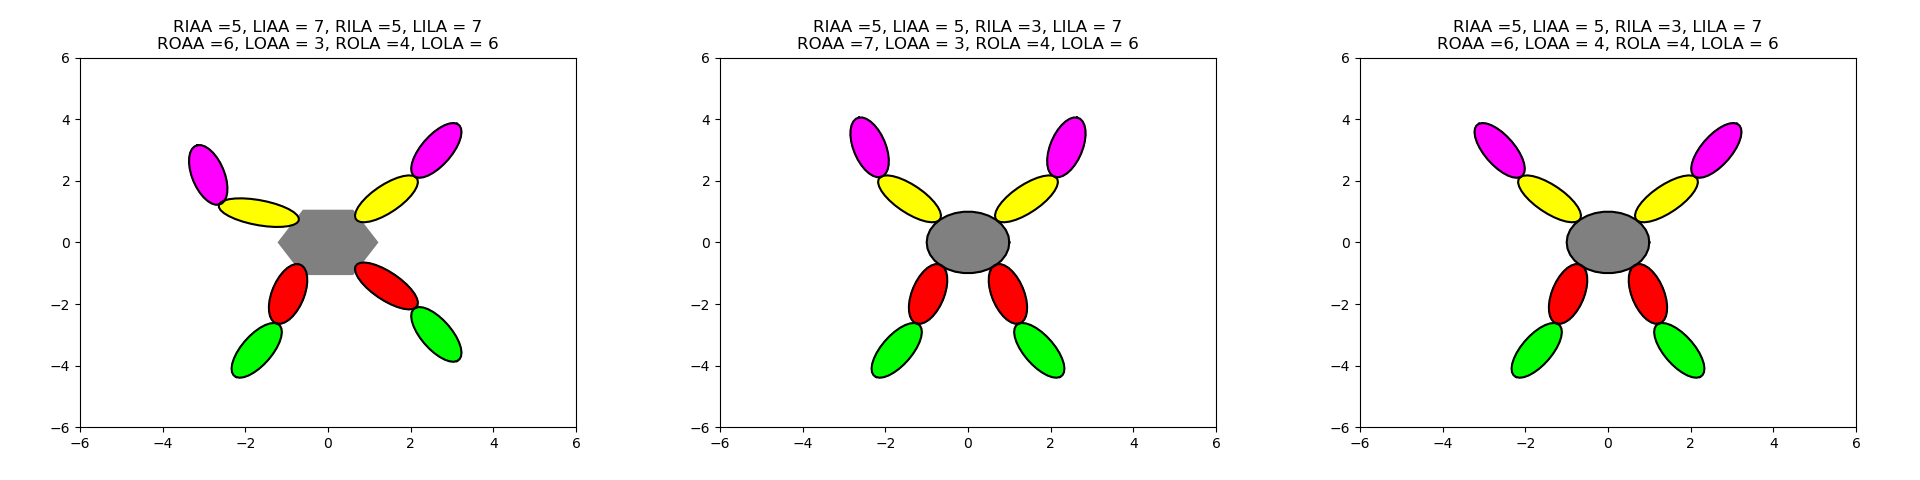
\includegraphics[width=180mm]{figs/mql_trial1_all.png}
	\caption{Observed (left), predicted (center), and actual (right) MQLs for trial one.}
\end{figure}
\begin{figure}[!ht]
	\centering
	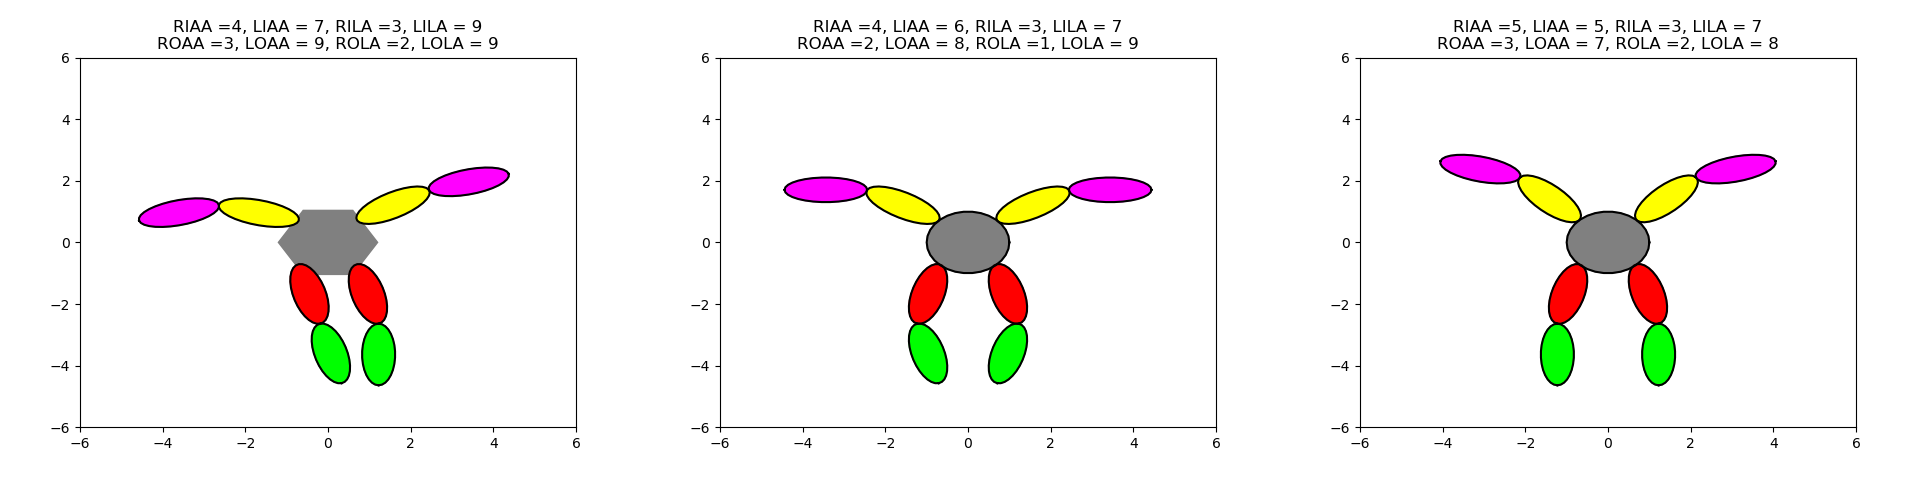
\includegraphics[width=180mm]{figs/mql_trial2_all.png}
	\caption{Observed (left), predicted (center), and actual (right) MQLs for trial two.}
\end{figure}
\begin{figure}[!ht]
	\centering
	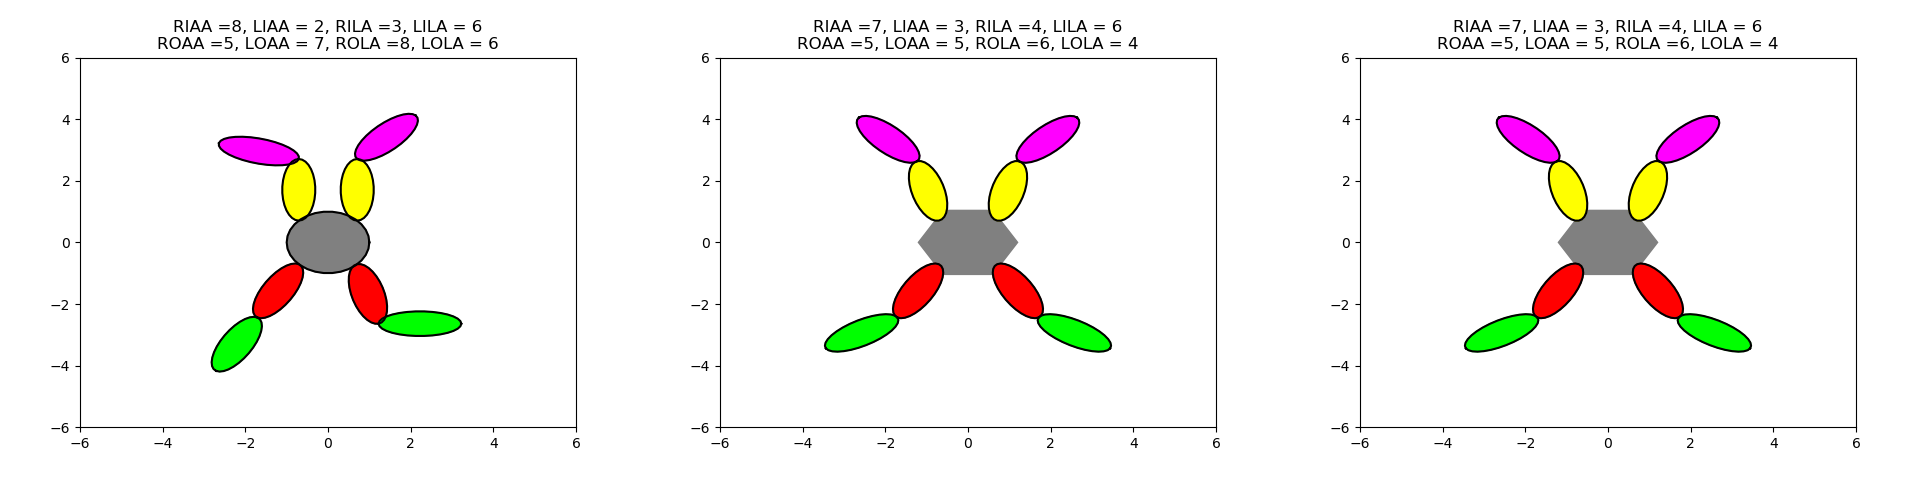
\includegraphics[width=180mm]{figs/mql_trial3_all.png}
	\caption{Observed (left), predicted (center), and actual (right) MQLs for trial three.}
\end{figure}
\begin{figure}[!ht]
	\centering
	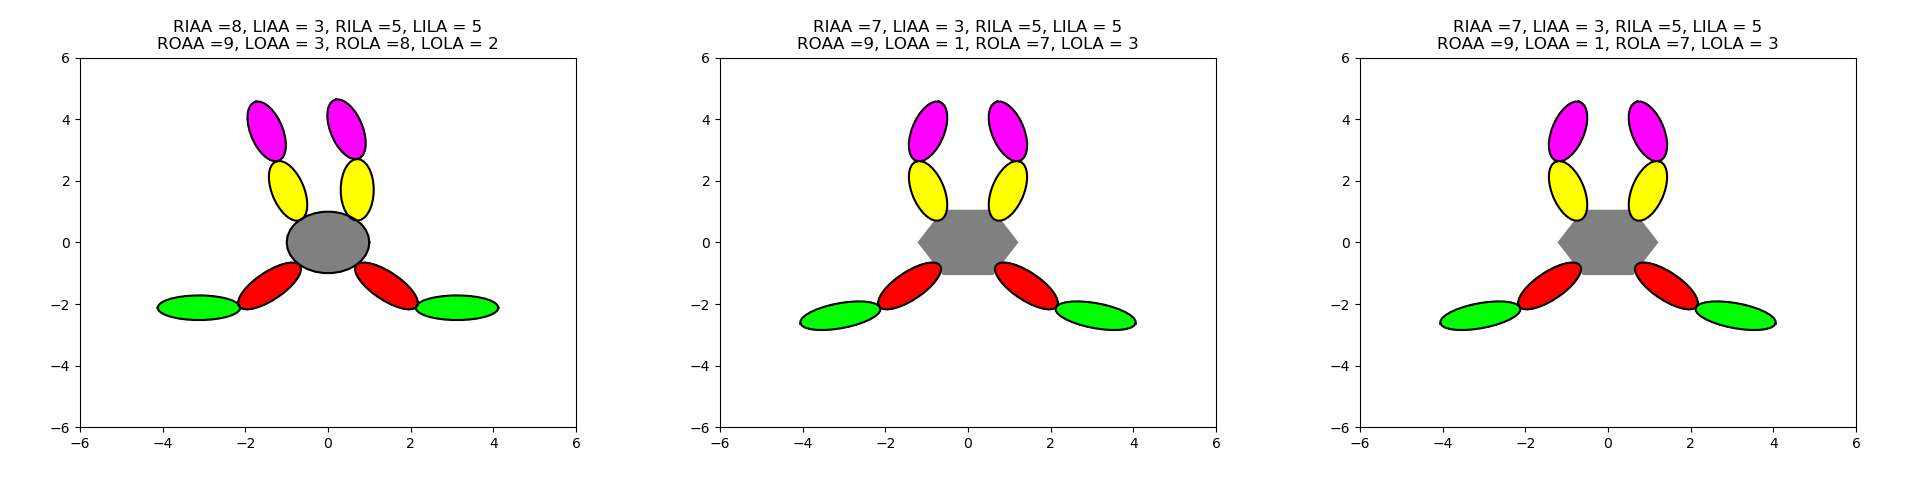
\includegraphics[width=180mm]{figs/mql_trial4_all.png}
	\caption{Observed (left), predicted (center), and actual (right) MQLs for trial four.}
\end{figure}
\begin{figure}[!ht]
	\centering
	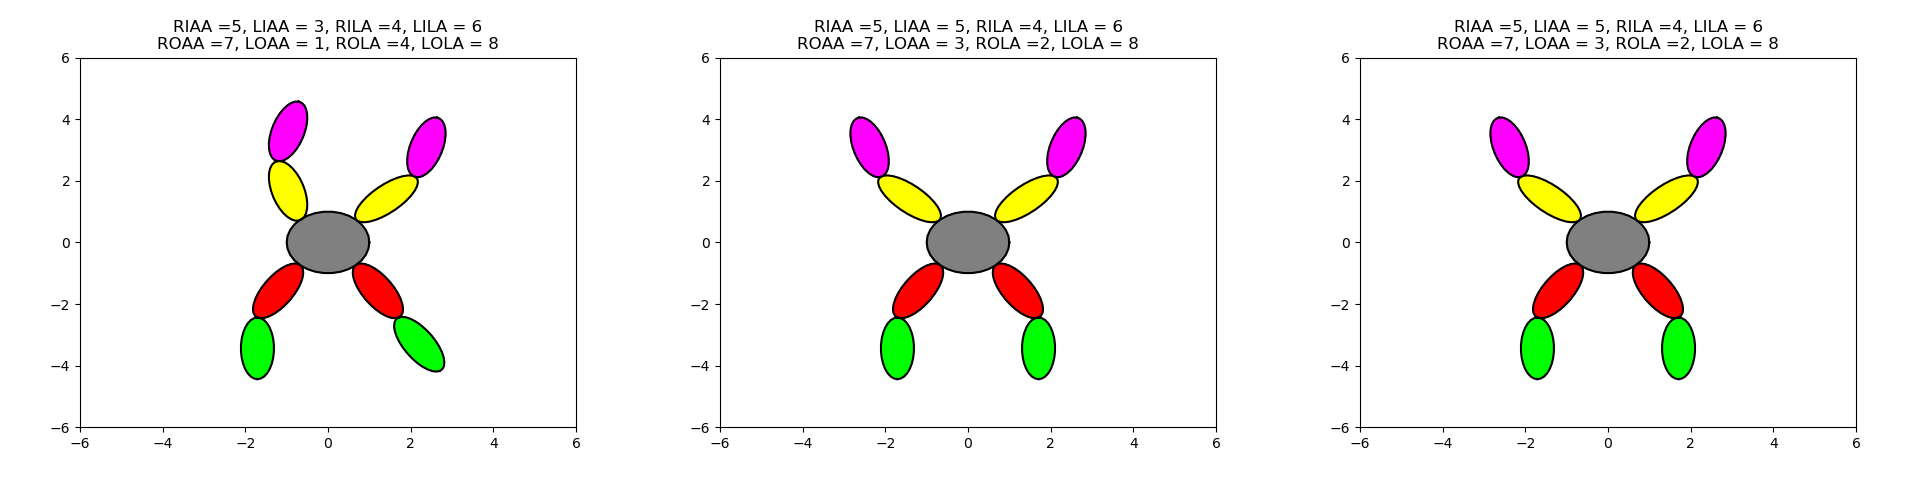
\includegraphics[width=180mm]{figs/mql_trial5_all.png}
	\caption{Observed (left), predicted (center), and actual (right) MQLs for trial five.}
\end{figure}
\begin{figure}[!ht]
	\centering
	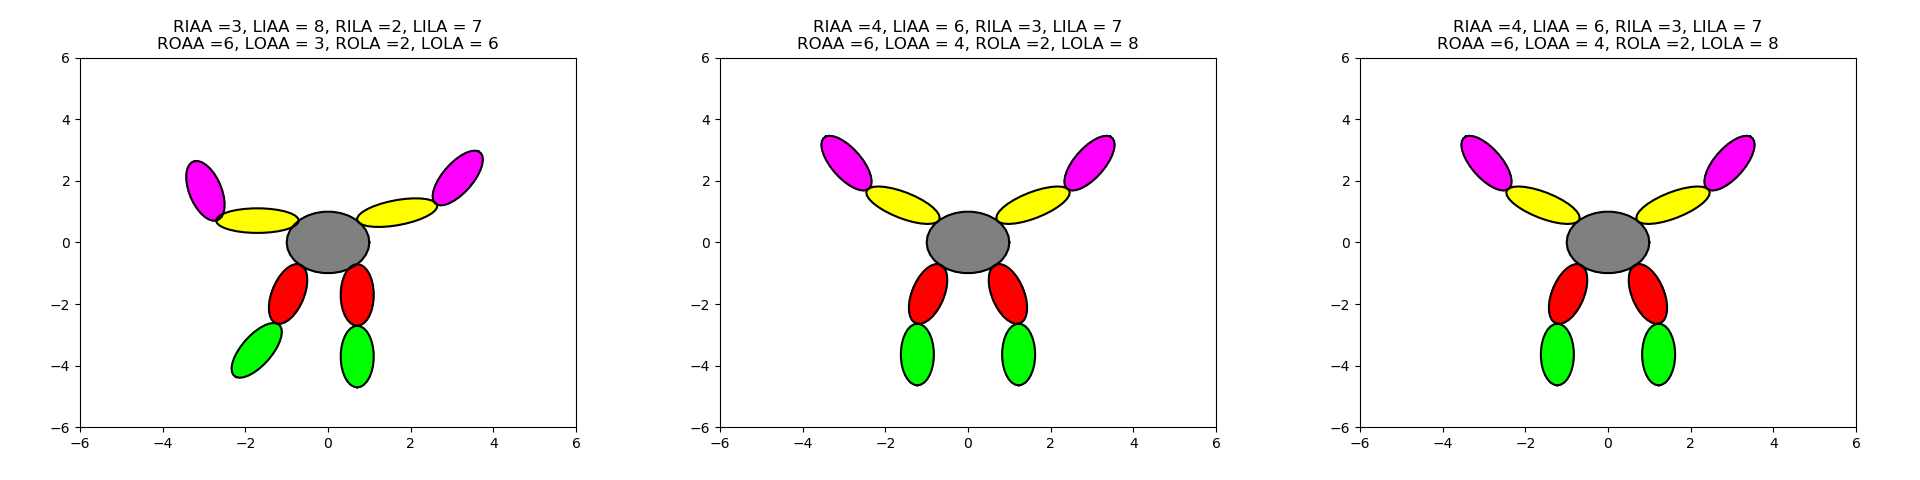
\includegraphics[width=180mm]{figs/mql_trial6_all.png}
	\caption{Observed (left), predicted (center), and actual (right) MQLs for trial six.}
\end{figure}
\begin{figure}[!ht]
	\centering
	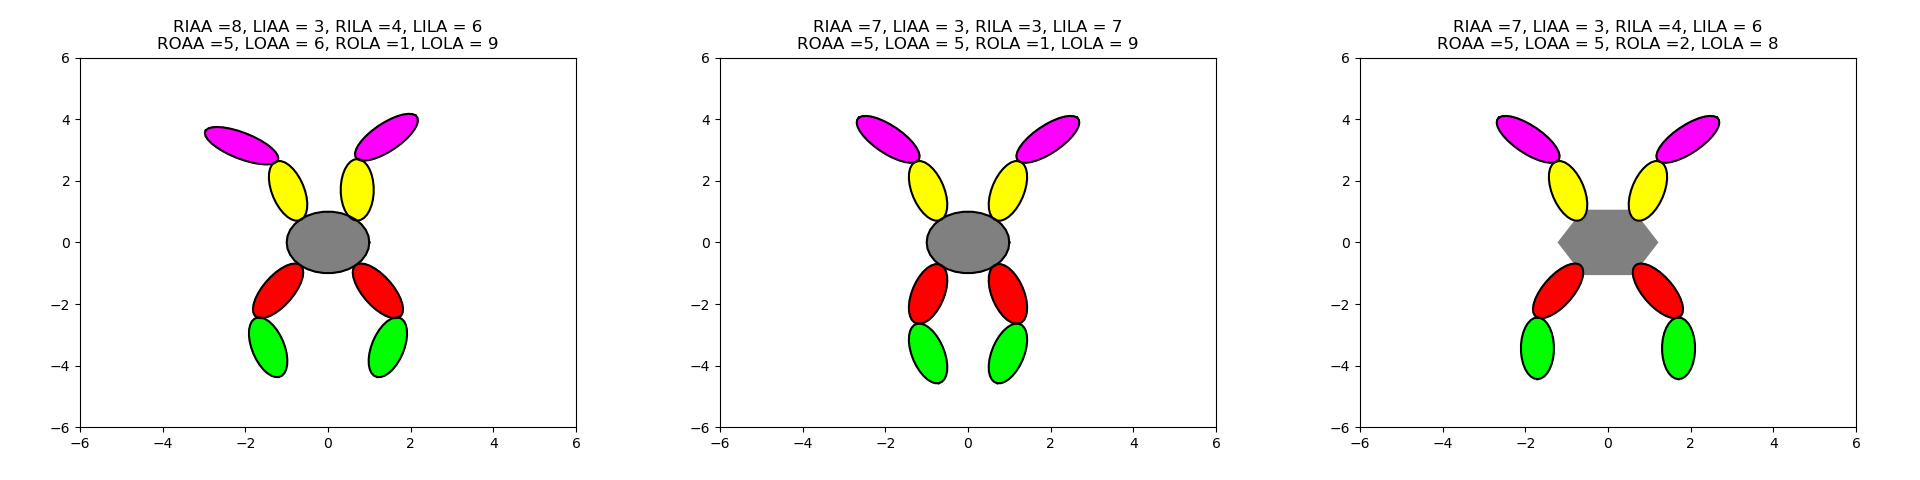
\includegraphics[width=180mm]{figs/mql_trial7_all.png}
	\caption{Observed (left), predicted (center), and actual (right) MQLs for trial seven.}
\end{figure}
\begin{figure}[!ht]
	\centering
	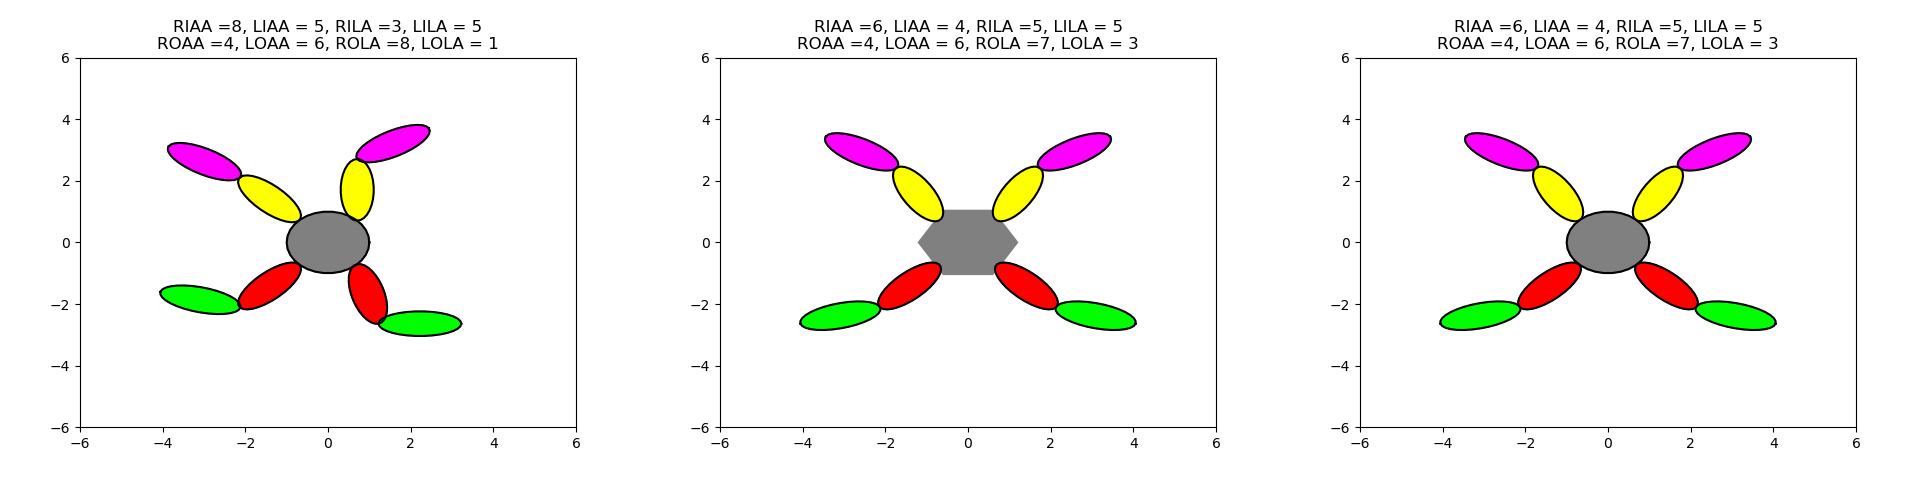
\includegraphics[width=180mm]{figs/mql_trial8_all.png}
	\caption{Observed (left), predicted (center), and actual (right) MQLs for trial eight.}
\end{figure}
\begin{figure}[!ht]
	\centering
	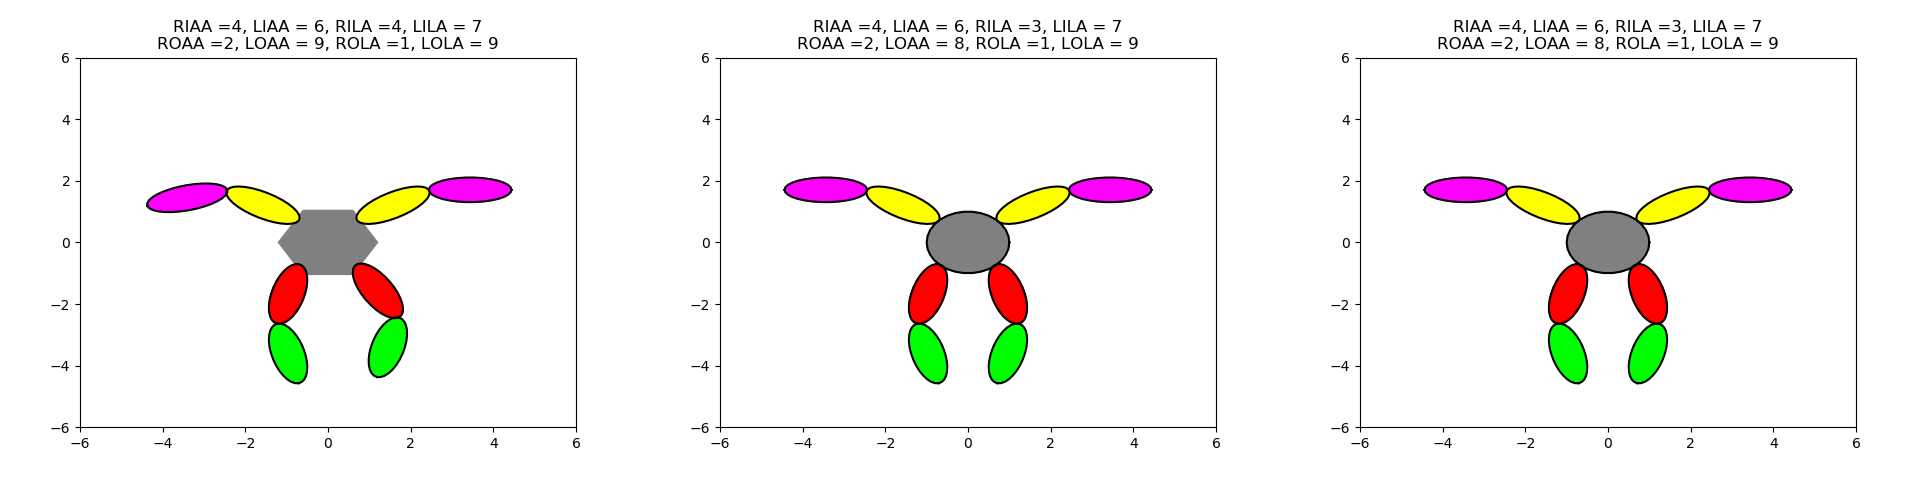
\includegraphics[width=180mm]{figs/mql_trial9_all.png}
	\caption{Observed (left), predicted (center), and actual (right) MQLs for trial nine.}
\end{figure}
\begin{figure}[!ht]
	\centering
	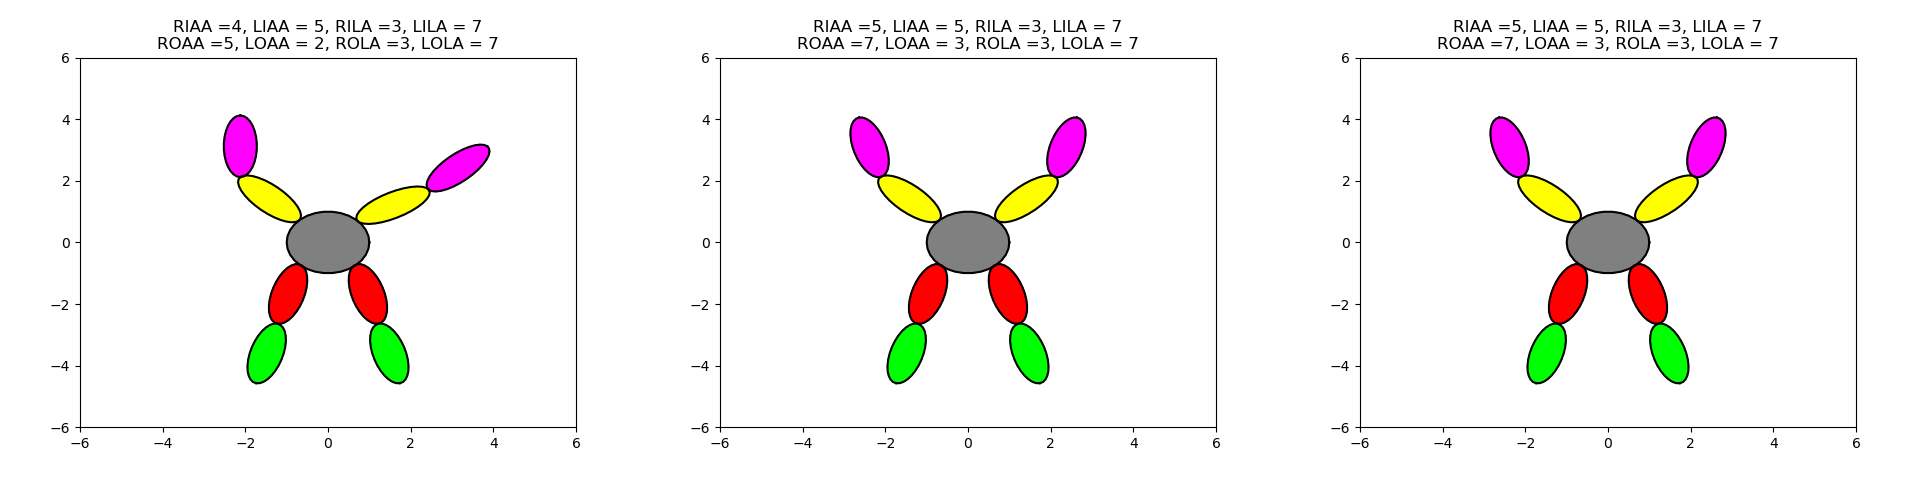
\includegraphics[width=180mm]{figs/mql_trial10_all.png}
	\caption{Observed (left), predicted (center), and actual (right) MQLs for trial ten.}
\end{figure}

~\\
~\\
~\\
~\\
~\\
~\\
~\\
~\\
~\\
~\\
~\\
~\\
~\\
~\\
~\\
~\\
~\\
~\\
~\\
~\\
~\\
~\\
~\\
~\\

\section{Q4}

The accuracy of max-sum was surprisingly high at 84\%, only 1\% behind max-sum. 
I was under the impression that providing the actual marginalized probabilites 
would be much more useful in determining the best configuration, but what I 
would consider the "greedy" approach (just taking the best) worked well. To 
understand this a little better, I think we can compare it to a similar 
situation. For any classifier, even if that classifier returns values for each 
class label in the form of a probability, we usually end up simply taking the 
max of the classes. In that case, it is our best guess, so it makes sense to do 
so. Similarly, just using the max value is our best guess, so it makes sense to 
do so in this situation as well.

\end{document}